% ----------------------------------------------------------------------
%  Pracovní úkoly
% ----------------------------------------------------------------------
\section{Pracovní úkoly}

\begin{enumerate}
\item Změřte voltampérové charakteristiky fotonek GKE, Phywe.

\item Rozborem charakteristik zjistěte, která z nich je vakuová a která je plynem plněná.

\item Změřte VA charakteristiky vakuové fotonky pro záporné hodnoty anodového napětí.

\item Zpracováním výsledků měření určete hodnotu Planckovy konstanty.
\end{enumerate}

% ----------------------------------------------------------------------
%  Teoretická část
% ----------------------------------------------------------------------
\section{Teoretická část}

Chyba je spočtena pomocí metody přenosu chyb \cite{bib:metoda-prenosu-chyb} jako

\begin{equation}
    \sigma = \sqrt{\sum^n_{i=1} \left( \frac{\partial f}{\partial x_i} \right)^2 \sigma^2_{x_i}}
\end{equation}

% ----------------------------------------------------------------------
%  Výsledky a zpracování měření
% ----------------------------------------------------------------------
\section{Výsledky a zpracování měření}

\subsection{Voltampérové charakteristiky}
Proměřili jsme voltampérové charakteristiky dvou fotonek GKE a Phywe v propustném směru, abychom určili zda se jedná o plynovou nebo vakuovou fotonku. Podle \cite{bib:zadani} jsme měřili v oboru -3 $V$ < $U_a$ < 100 $V$ s krokem 0,5 $V$ na rozsahu 200 $nA$. Vzorek jsme osvětlovali pomocí rtuťové výbojky s použitým filtrem s vlnovou délkou 546 nm. Naměřené závislosti jsou znázorněny v obrázku \ref{fig:VA-char}.

\begin{figure}[!h]
    \centering
    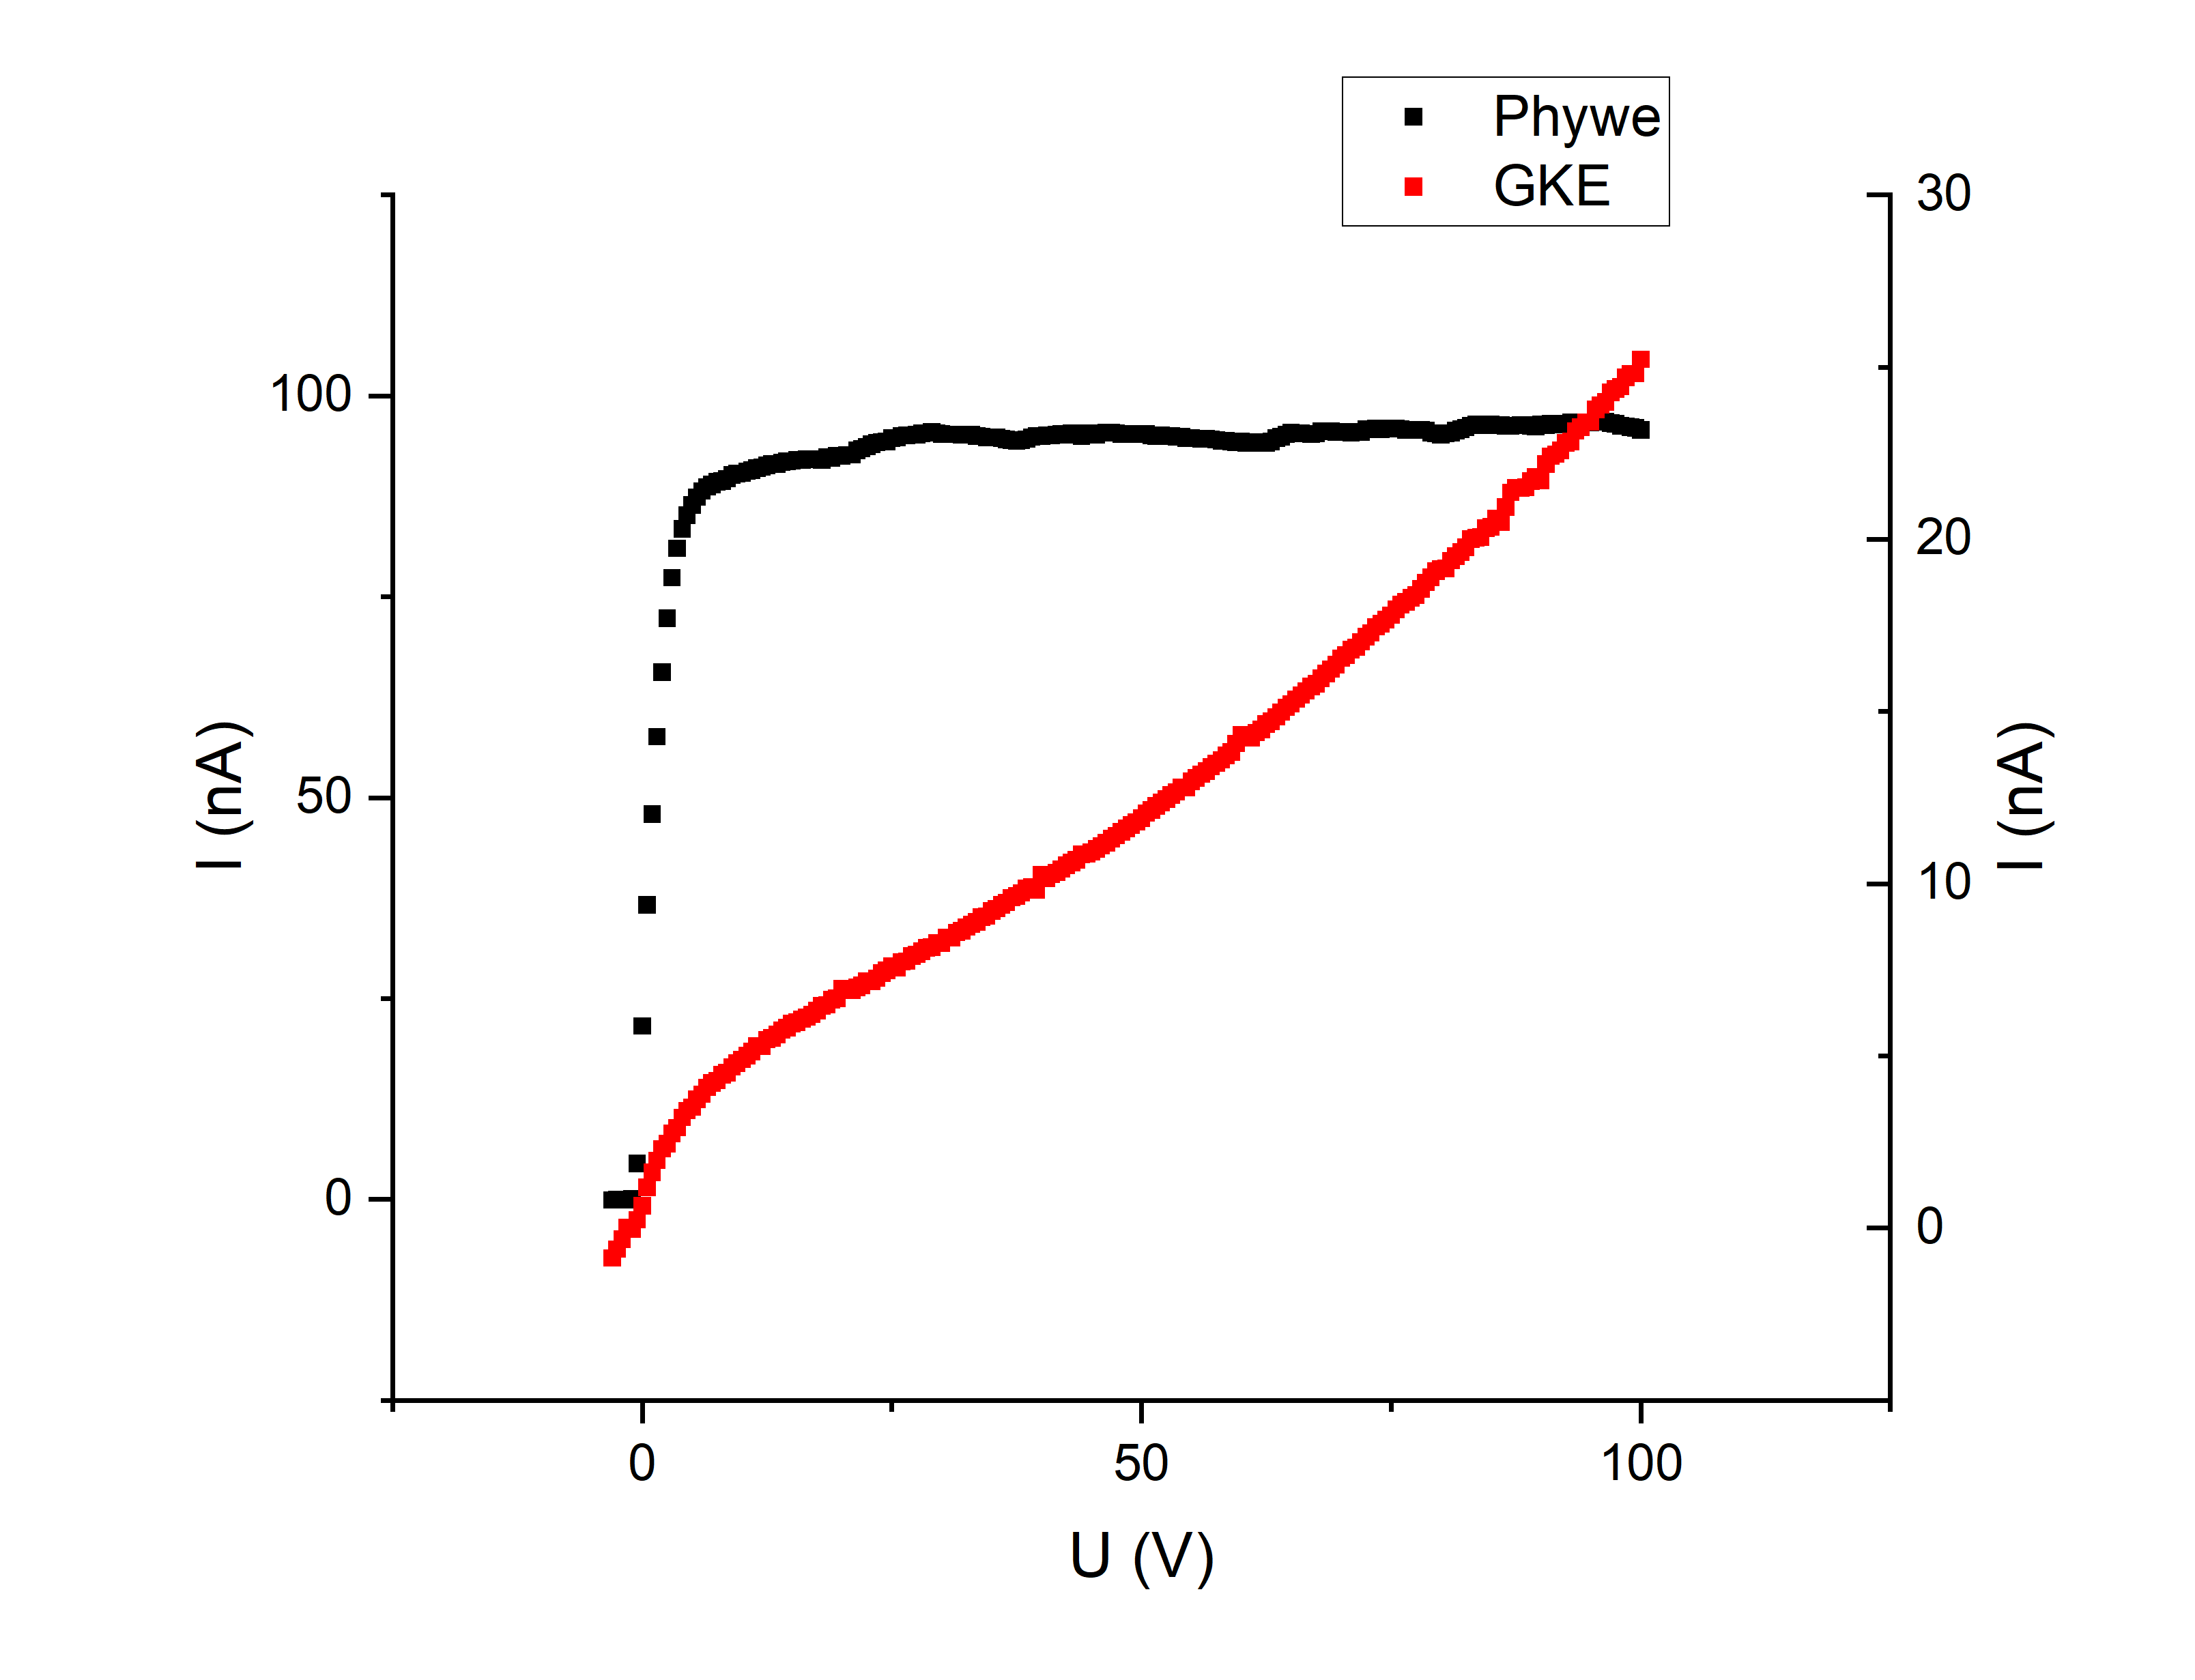
\includegraphics[width=1\linewidth]{A9 - Planck/VA charakteristiky.png}
    \caption{Voltampérové charakteristiky fotonek Phywe a GKE}
    \label{fig:VA-char}
\end{figure}

Na základě těchto závislostí jsme označili fotonku GKE jako plynovou a Phywe jako vakuovou. U fotonky GKE pozorujeme u nízkých hodnot napětí zlom v nárůstu proudu a poté monotónní růst proudu s napětím. To je způsobeno lavinovou ionizací plynu ve fotonce. Naopak u vakuové fotonky Phywe pozorujeme dosažení určité hodnoty proudu, která se již nezvyšuje s rostoucím napětím.

\subsection{Určení Planckovy konstanty}

Pro měření Planckovy konstanty jsme měřili v závěrném směru s vakuovou fotonkou Phywe (proč jsme zvolili tuto fotonku, viz. diskuze). Opět jsme jako zdroj osvětlení použili rtuťovou výbojku. Měnili jsme použité filtry tak, abychom proměřili závislost pro různé vlnové délky, konkrétně 365, 405, 436, 546 a 577 nm.

Měřili jsme v rozsahu -0,5 $V$ > $U_a$ > -3 $V$ s krokem pouze 0,05 V. Všechny naměřené závislosti jsou zobrazeny na obrázku.

U všech charakteristik jsme pozorovali určitou hodnotu nasyceného proudu $I_s$. V části grafu před saturací jsme vybrali přibližně 5 bodů pro každou závislost a tuto oblast jsme fitovali lineární regresí s předpisem $y = a\cdot x + b$. Průsečík této přímky s hodnotou nasyceného proudu $I_s$ jsme označili jako kritické napětí $V_0$. Tento postup je zobrazen na obrázku \ref{fig:V0}.

\begin{figure}[!h]
    \centering
    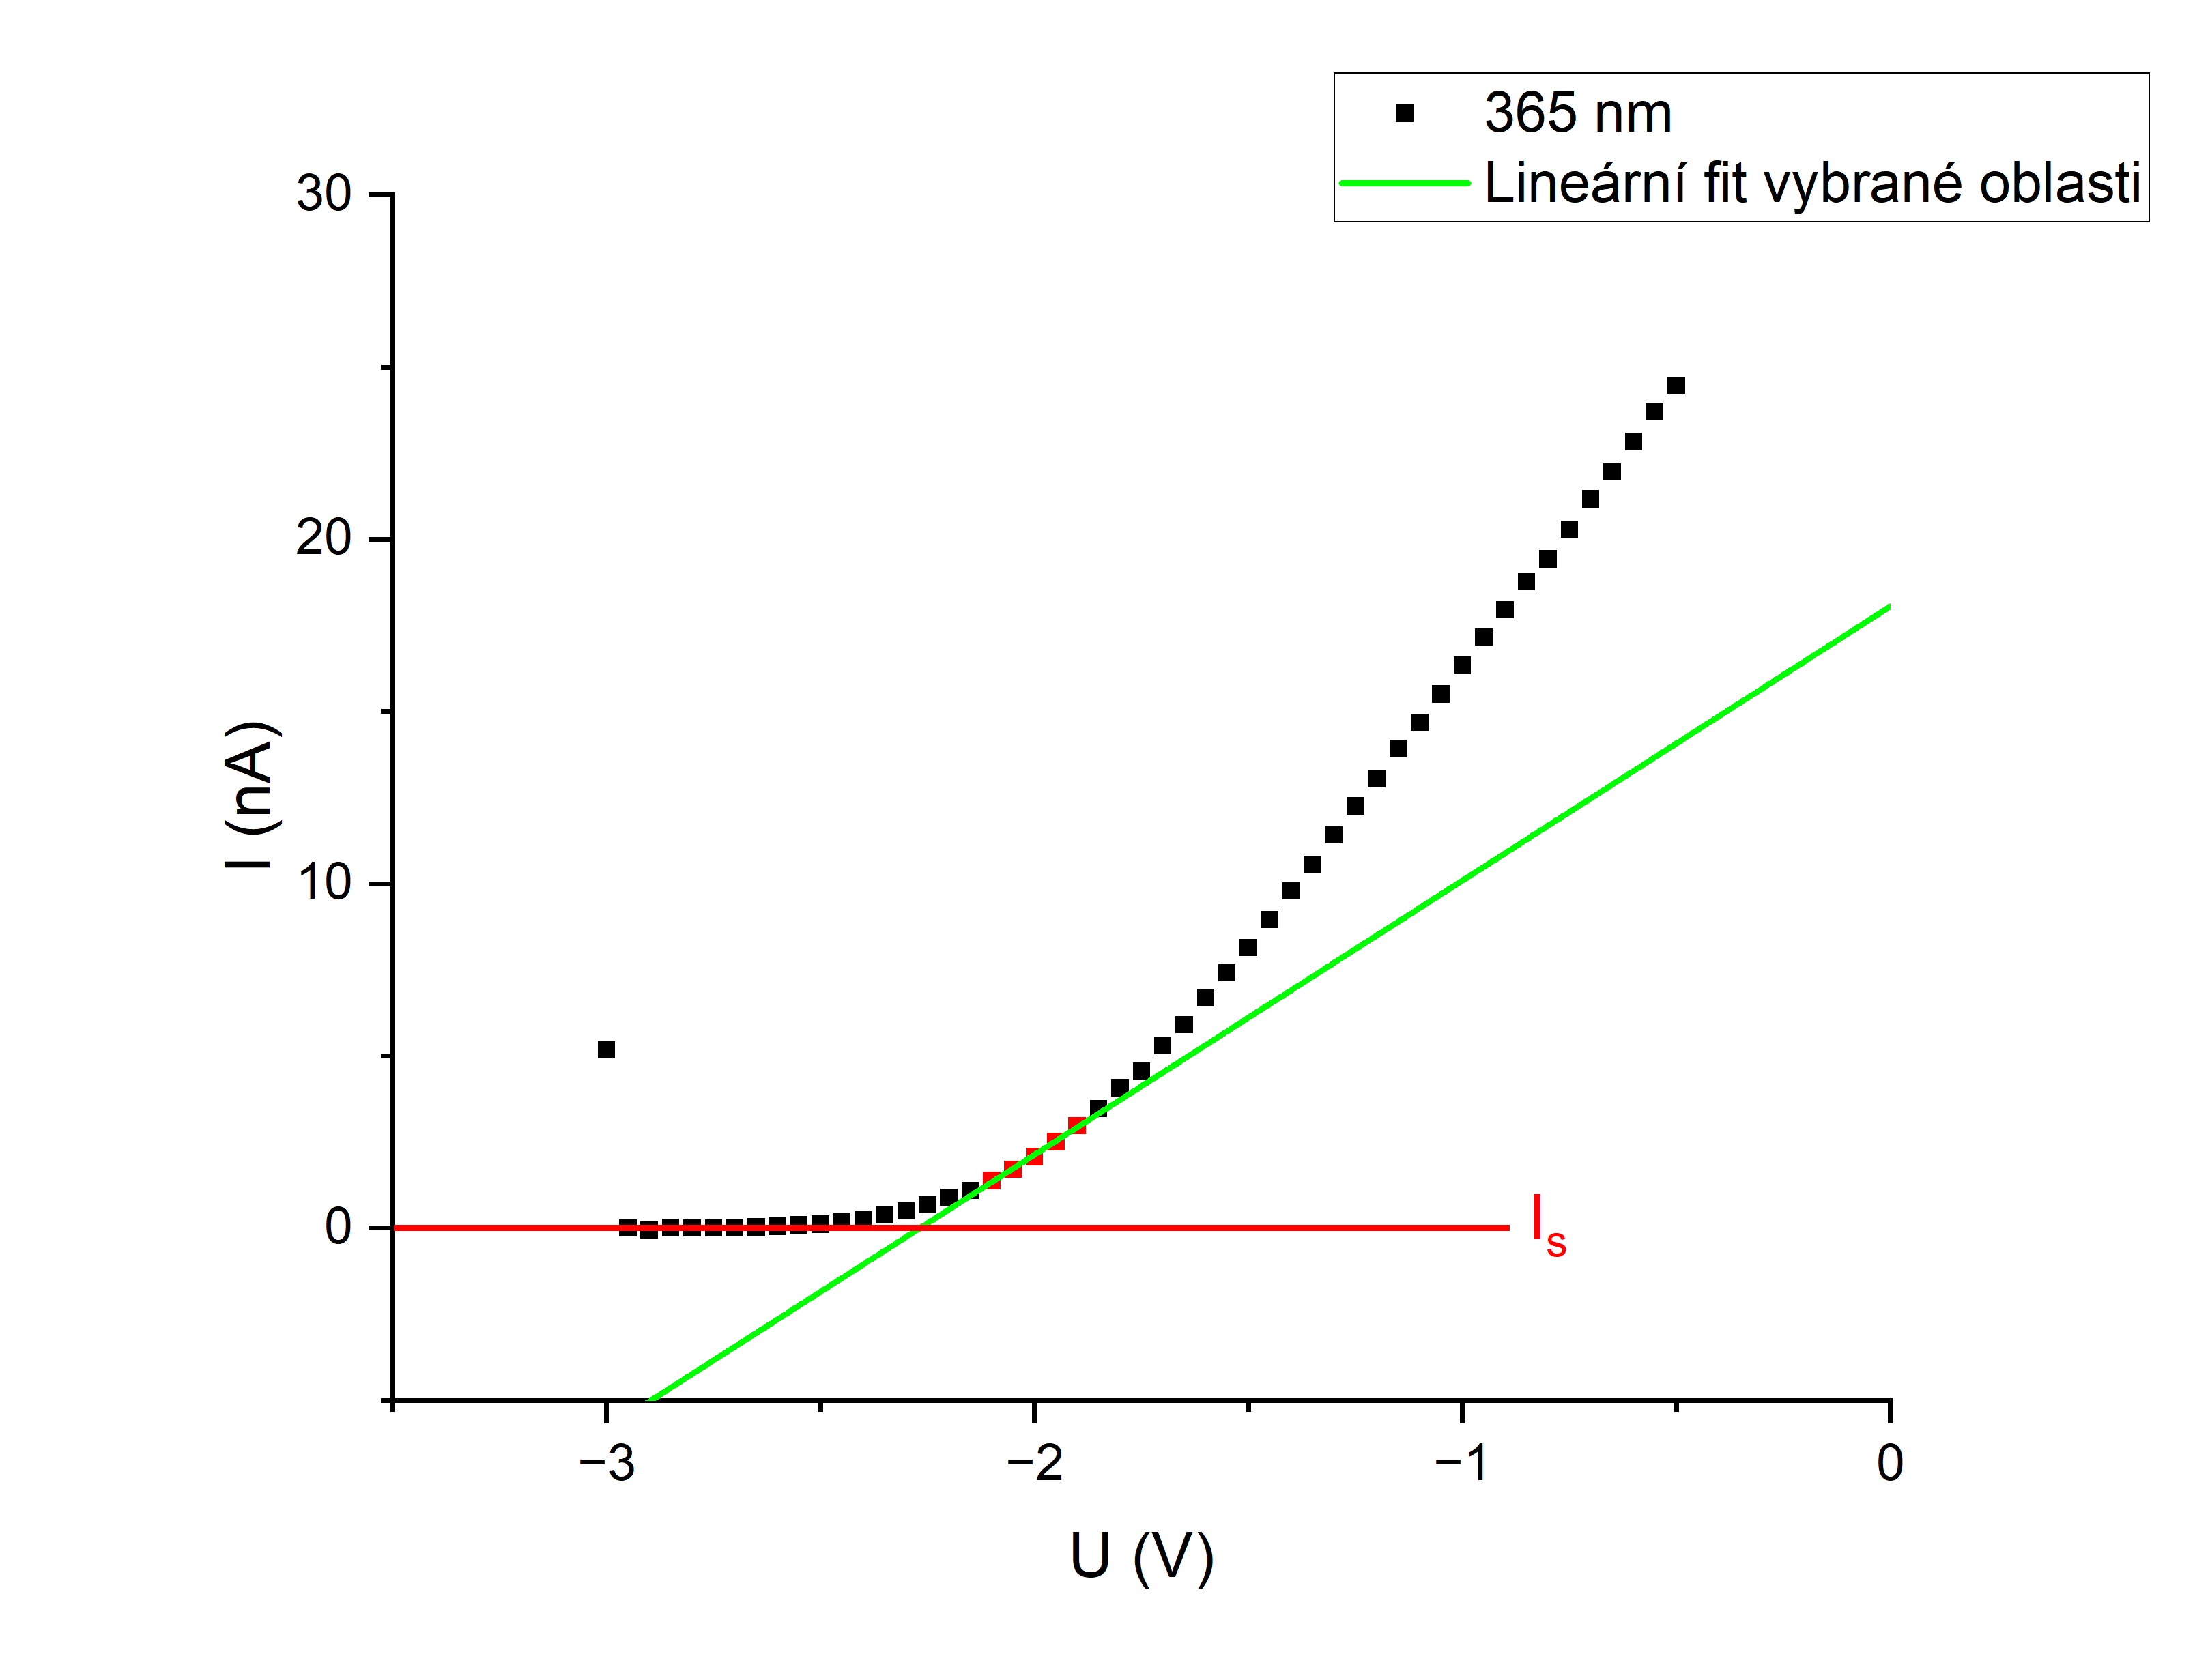
\includegraphics[width=1\linewidth]{A9 - Planck/Výpočet V0.png}
    \caption{Postup určení kritického napětí}
    \label{fig:V0}
\end{figure}

Analogicky jsme spočítali hodnoty kritického napětí pro všechny vlnové délky. Jednotlivé závislosti jsou zobrazeny na obrázku \ref{fig:V-lambda}.

\begin{figure}[!h]
    \centering
    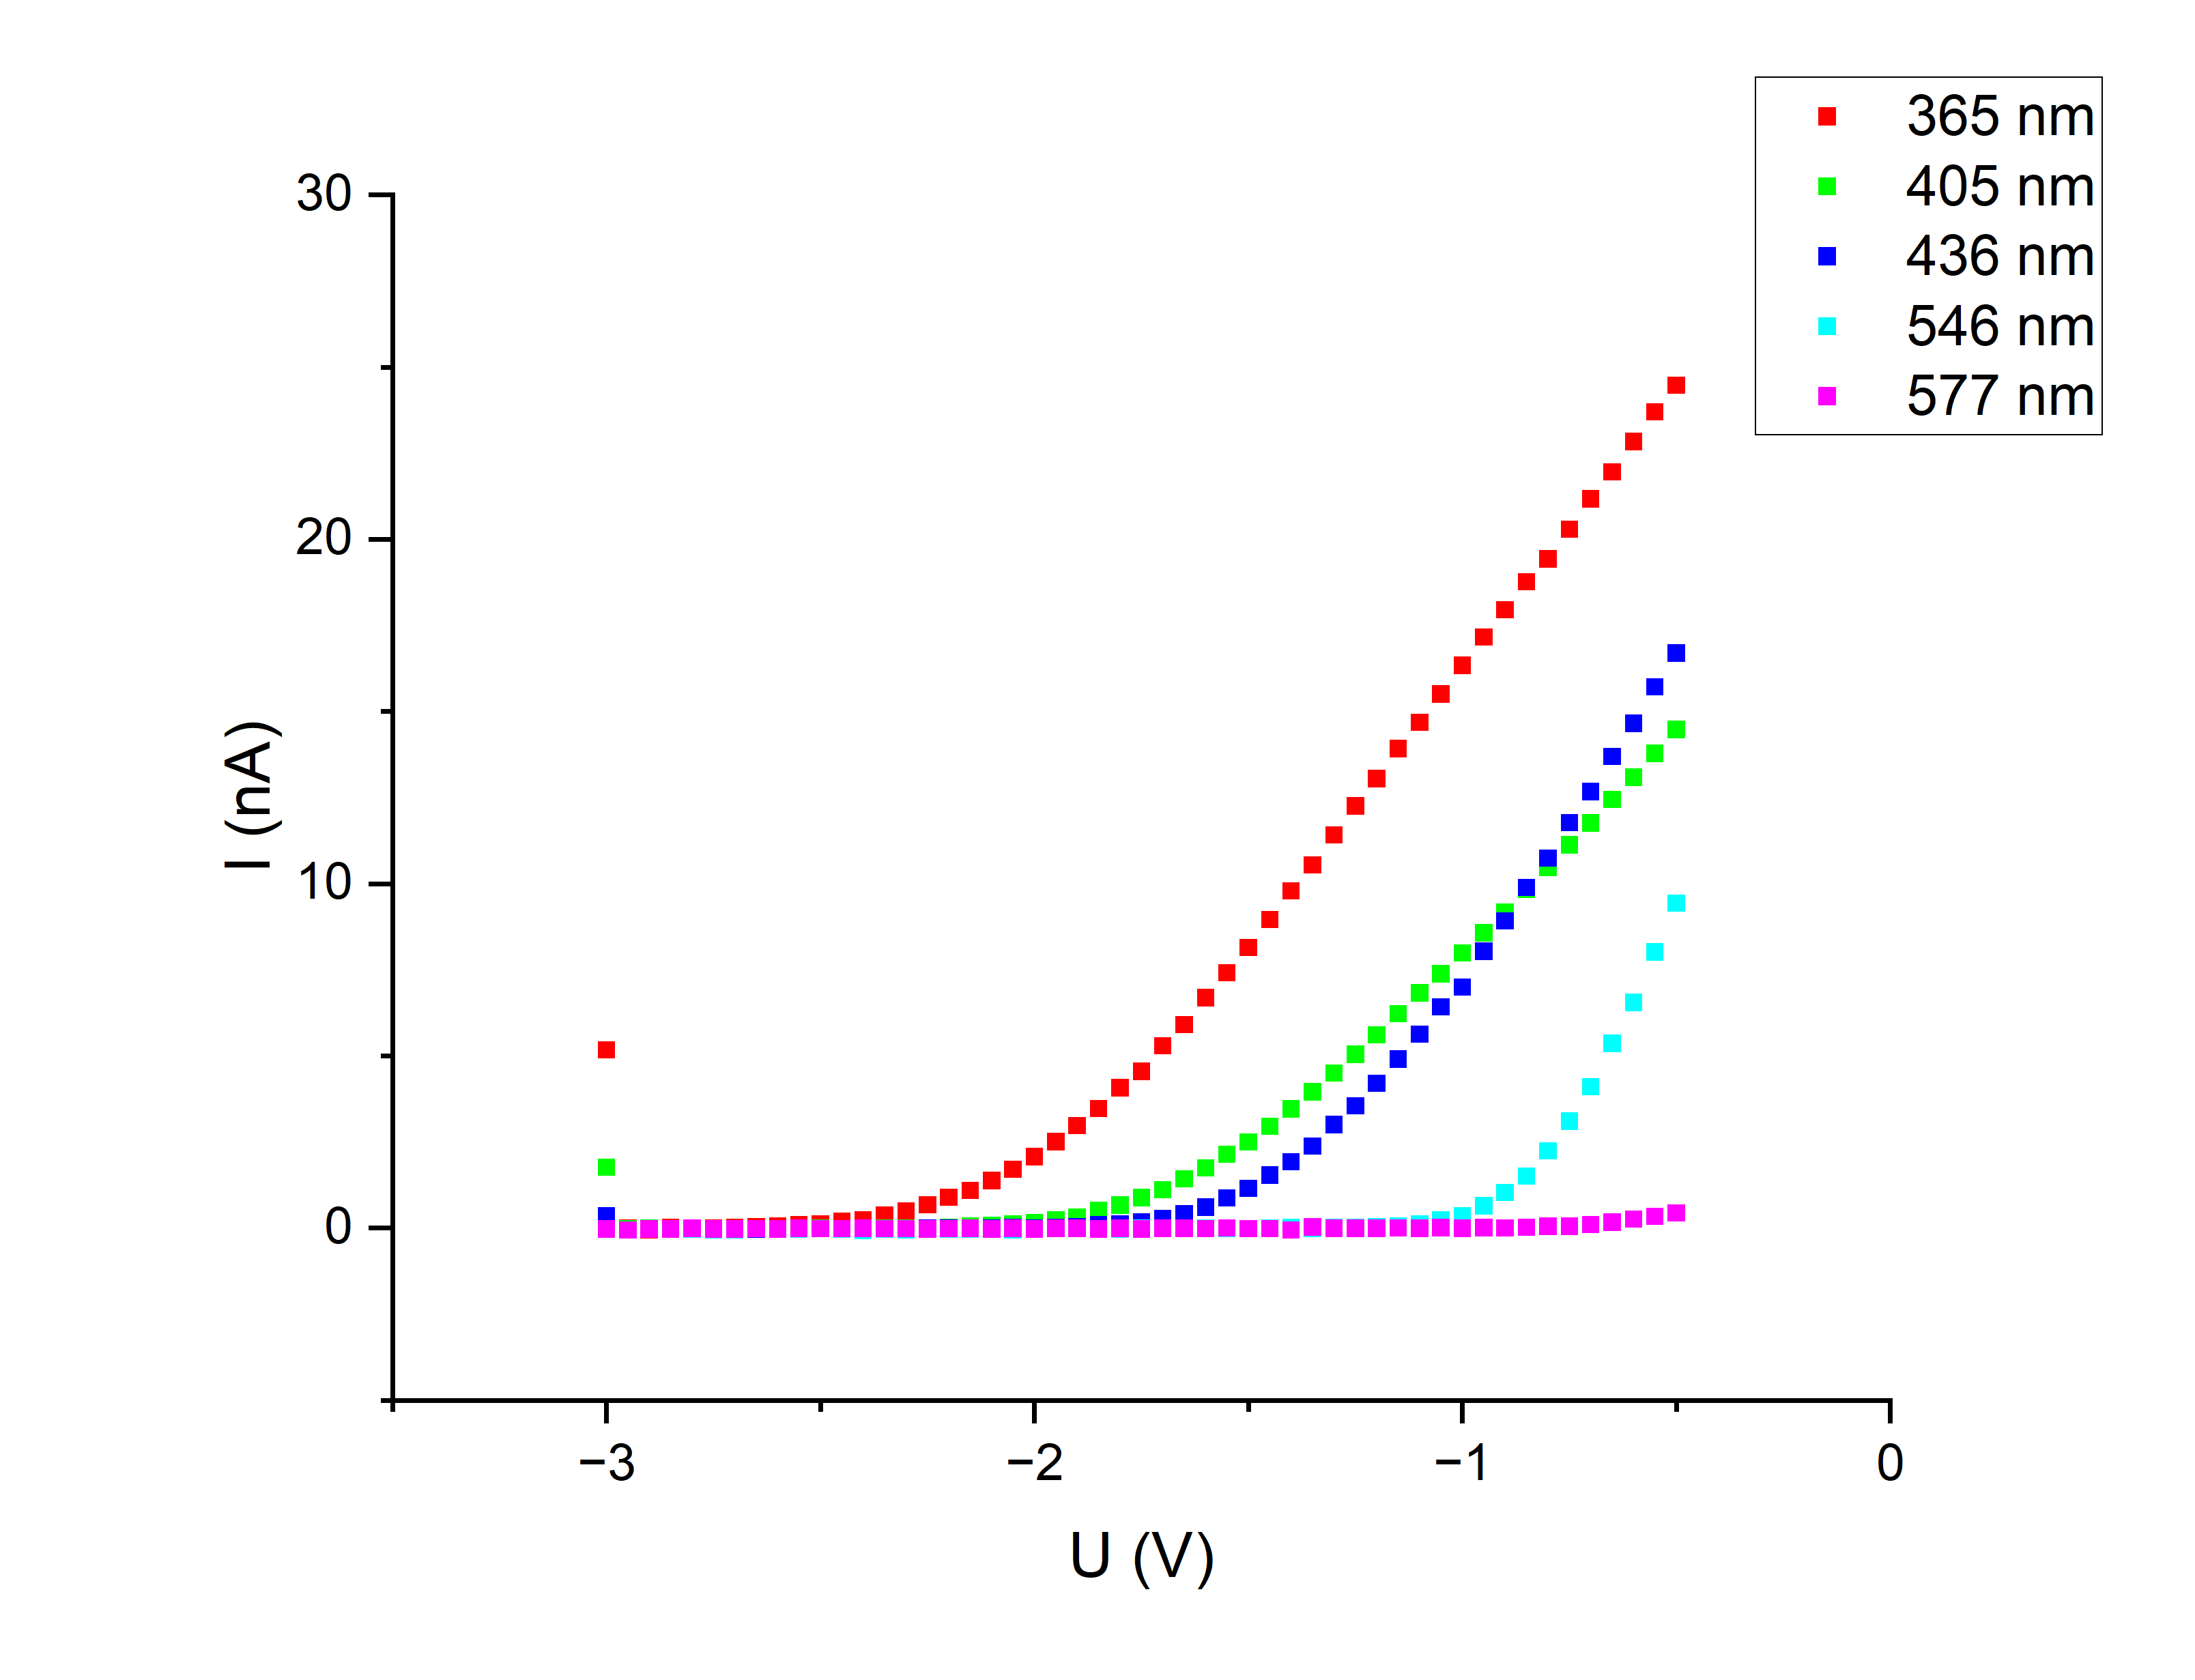
\includegraphics[width=1\linewidth]{A9 - Planck/Všechny vlnové délky.png}
    \caption{Závislost kritického napětí na vlnové délce}
    \label{fig:V-lambda}
\end{figure}

Nejistota kritického napětí je způsobena nepřesností měřidla v kombinaci s chybou při zpracování dat (statistická chyba a interpolace). Měřili jsme s přístrojem Keithley 6487, jehož nejistota je popsána na straně 255 ve specifikacích přístroje na \cite{bib:pristroj}. Chybou při zpracování dat se rozumí statistická chyba, kterou můžeme považovat za zanedbatelnou vůči chybě vzniklé při interpolaci naměřených dat, kterou do této skupiny také zahrnujeme. Experimentátor má určitou volnost při výběru konkrétních hodnot pro lineární fit. Tato nejistota byla odhadnuta jako změna kritického napětí při výběru jiného počtu dat nebo jiných hodnot, které by zároveň stále splňovaly požadované kritéria na lineární fit. Celková nejistota je poté určena jako součet druhých mocnin těchto dvou nejistot pod odmocninou. Odtud jsme nejistotu pro všechny vlnové délky odhadli na 0,1 $V$ kromě vlnové délky 577 $nm$, kde byla pozorována určitá fluktuace naměřených dat, proto jsme nejistotu odhadli na 0,2 $V$. Dopočtené hodnoty jsou znázorněné v tabulce \ref{tab:krit-nap}.

\begin{table}[!h]
\centering
\caption{Kritické napětí pro jednotlivé vlnové délky}
\label{tab:krit-nap}
\begin{tabular}{cccc}
\hline
$\lambda$ / nm & $\nu$ / ($10^{14}$ Hz) & $E_k$ / eV & $\sigma(V_0)$ / V \\
\hline
405 & 7,41 & 1,951 & 0,1 \\
365 & 8,22 & 2,267 & 0,1 \\
436 & 6,88 & 1,689 & 0,1 \\
546 & 5,49 & 1,072 & 0,1 \\
577 & 5,20 & 0,788 & 0,2 \\
\hline
\end{tabular}
\end{table}

Závislost kritického napětí na vlnové délce je zobrazena na obrázku.



% ----------------------------------------------------------------------
%  Diskuse výsledků
% ----------------------------------------------------------------------			
\section{Diskuse výsledků}

Proč nemůžeme měřit s plynovou fotonkou Placka?

Divné body vlevo na grafu.

Výběr bodů pro linární fit.

% ----------------------------------------------------------------------
%  Závěr
% ----------------------------------------------------------------------
\section{Závěr}
